\section[Основные положения теории нечеткого логического вывода]{%
  ОСНОВНЫЕ ПОЛОЖЕНИЯ ТЕОРИИ \\
  НЕЧЕТКОГО ЛОГИЧЕСКОГО ВЫВОДА
}

\subsection{Нечеткое множество}

\emph{Нечеткое множество} определяется как множество упорядоченных пар вида
\[
A = \{ \mu_A(x) / x \},
\]
где
\( x \) --- элемент универсального множества \( E \);
\( \mu_A(x) \) --- характеристическая функция принадлежности,
принимающая значения в интервале \( [0, 1] \).

\emph{Функция принадлежности} указывает степень принадлежности
элемента \( x \) множеству \( A \).
Существуют различные способы задания нечеткого множества и,
соответственно, функции принадлежности. Как и в обычном случае,
нечеткое множество можно задавать путем перечисления его элементов, например:
\[
  A = \{ 0{,}3/x_1, 0{,}7/x_2, \ldots, 0{,}5/x_9 \}.
\]
Данное множество содержит девять элементов, при этом его второй элемент \( x_2 \)
принадлежит ему со степенью \( 0{,}7 \).
Кроме этого, нечеткое множество можно определить путем аналитического описания его
функции принадлежностей \( \mu_A(x) \).
В научном сообществе исследовано большое число таких функций,
среди которых наиболее наибольшей популярностью пользуются
треугольная и трапециедальная, колоколообразная и Гауссова функции,
а также сигмоидальные, линейные,
квадратичные и гармонические Z(S)-сплайны\cite{fuzzy_bstu_22}.

Использование функции принадлежности позволяет связать
\emph{лингвистическую переменную}, описывающую положение дел на естественном языке,
с её нечетким численным представлением.
Например, пусть
\( E = \{ \text{Запорожец}, \text{Жигули}, \text{Мерседес}, \ldots \} \) ---
множество марок автомобилей, а
\( E' = [0, \infty) \) --- универсальное множество <<Стоимость>>,
тогда на \( E' \) можно определить нечеткие множества типа
<<Для бедных>>, <<Для среднего класса>>, <<Престижные>> с
соответствующими функциями принадлежности,
как показано на рисунке~\ref{fig:example_functions}.

\begin{figure}[h!]
  \centering
  \fcolorbox{gray}{white}{
    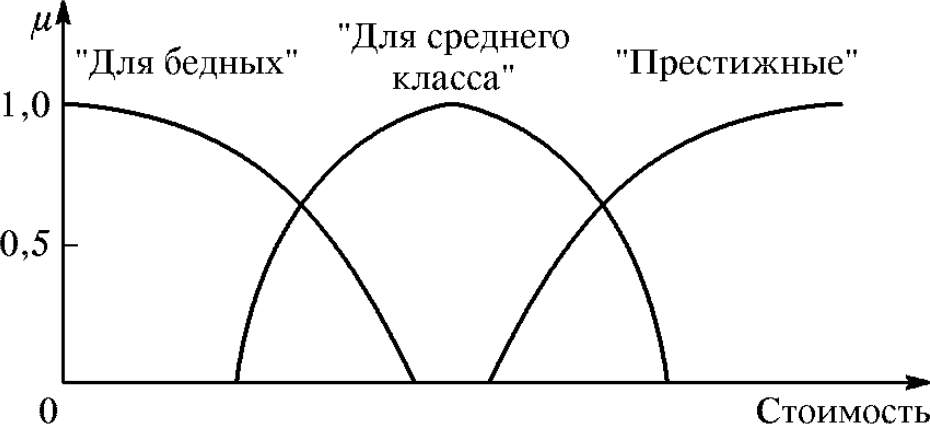
\includegraphics[width=120mm]{fig/example_functions}
  }
  \caption{Примеры функций принадлежности}
  \label{fig:example_functions}
\end{figure}

Располагая данными функциями, а также стоимостями автомобилей из \( E \) в
данный момент времени, мы можем определить на \( E' \) нечеткие множества
с такими же названиями. Так, например, нечеткое множество <<Для бедных>>,
заданное на \( E = \{ \text{Запорожец}, \text{Жигули}, \text{Мерседес}, \ldots \} \),
выглядит так, как показано на рисунке~\ref{fig:example_set}.

\begin{figure}[h!]
  \centering
  \fcolorbox{gray}{white}{
    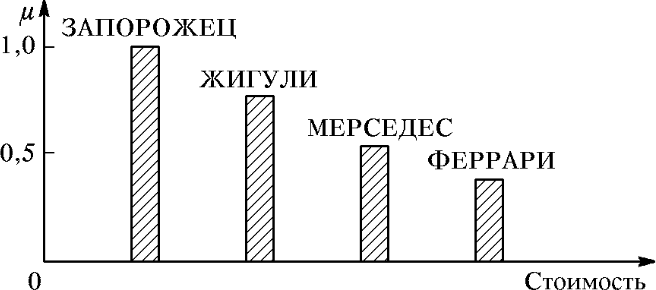
\includegraphics[width=120mm]{fig/example_set}
  }
  \caption{Пример задания нечеткого множества}
  \label{fig:example_set}
\end{figure}

Аналогично можно определить нечеткое множество
<<Скоростные>>, <<Средние>>, <<Тихоходные>> и~т.~д.~\cite{kruglov2001}.

\pagebreak

\subsection{Операции над нечеткими множествами}

Перечислим основные операции над нечеткими множествами.
Пусть \( A, B, C, D \) --- нечеткие множества на универсальном множестве \( E \).
Тогда говорят, что \( A \) \emph{содержится} в \( B \) (\( A \subset B \)),
если \( \forall x \in E: \mu_A(x) \le \mu_B(x) \).

Нечеткие множества \( A \) и \( B \) \emph{равны} (\( A = B \)), если
\( \forall x \in E: \mu_A(x) = \mu_B(x) \).

Нечеткое множество \( A \) \emph{дополняет} \( B \) (\( A = \overline{B}, B = \overline{A} \)),
если \( \forall x \in E: \mu_A(x) = 1 - \mu_B(x) \).

\emph{Пересечением} нечетких множеств \( A \) и \( B \) называется множество
\( C = A \cap B \), определяемое в общем случае как
\[ C = \{ \mu_C(x) / x \}, \mu_C(x) = T(\mu_A(x), \mu_B(x)), \]
где \( T: [0, 1] \times [0,1] \rightarrow [0, 1] \) ---
двуместная действительная функция, называемая \emph{t-нормой},
удовлетворяющая следующим условиям:
\begin{itemize}
\item \( T(0, 0) = 0; \; T(\mu_A, 1) = \mu_A; \; T(1, \mu_B) = \mu_B \);
\item \( \mu_A \le \mu_C, \mu_B \le \mu_D \rightarrow T(\mu_A, \mu_B) \le T(\mu_C, \mu_D) \);
\item \( T(\mu_A, \mu_B) = T(\mu_B, \mu_A) \);
\item \( T(\mu_A, T(\mu_B, \mu_C)) = T(T(\mu_A, \mu_B), \mu_C)) \).
\end{itemize}

На практике в качестве t-нормы часто используют операции
нахождения минимума \( \min(\mu_A, \mu_B ) \),
произведения \( \mu_A \cdot \mu_B \), а также
\( \max(0, \mu_A + \mu_B - 1) \).

\emph{Объединением} нечетких множеств \( A \) и \( B \) называется множество
\( C = A \cup B \), определяемое в общем случае как
\[ C = \{ \mu_C(x) / x \}, \mu_C(x) = S(\mu_A(x), \mu_B(x)), \]
где \( S: [0, 1] \times [0,1] \rightarrow [0, 1] \) ---
двуместная действительная функция (\emph{t-конорма}),
удовлетворяющая следующим условиям:
\begin{itemize}
\item \( S(1, 1) = 1; \; S(\mu_A, 0) = \mu_A; \; S(0, \mu_B) = \mu_B \);
\item \( \mu_A \ge \mu_C, \mu_B \ge \mu_D \rightarrow S(\mu_A, \mu_B) \ge S(\mu_C, \mu_D) \);
\item \( S(\mu_A, \mu_B) = S(\mu_B, \mu_A) \);
\item \( S(\mu_A, S(\mu_B, \mu_C)) = S(S(\mu_A, \mu_B), \mu_C)) \).
\end{itemize}

На практике в качестве t-конормы часто используют операции
нахождения максимума \( \max(\mu_A, \mu_B ) \),
\( \mu_A + \mu_B - \mu_A \mu_B \), а также
\( \min(1, \mu_A + \mu_B) \).

\pagebreak

\subsection{Схема алгоритмов нечеткого вывода}

Пусть имеется предварительно составленный экспертом набор нечетких правил вида: \par
\( \text{П}_1 \): если \( x_1 \) есть \( A_1 \), то \( y \) есть \( B_1 \), \par
\( \text{П}_2 \): если \( x_2 \) есть \( A_2 \), то \( y \) есть \( B_2 \), \par
..........................................................  \par
\( \text{П}_n \): если \( x_n \) есть \( A_n \), то \( y \) есть \( B_n \), \\
где \( x \) --- входная переменная,
\( y \) --- переменная вывода,
\( A \) и \( B \) --- функции принадлежности,
определенные соответственно на \( x \) и \( y \).

Прямой нечеткий логический вывод в общем случае осуществляется в
соответствии с алгоритмом, состоящем из следующих четырех этапов:
\begin{enumerate}
\item Приведение к нечеткости, или \emph{фазификация}.
  Функции принадлежности, определенные на входных переменных,
  применяются к их фактическим значениям для определения степени
  истинности каждой предпосылки каждого правила.
\item \emph{Логический вывод}.
  На основании значений истинности предпосылок и выбранной t-конормы вычисляются
  значения истинности условной части каждого правила.
  Полученные значения истинности применяются к заключениям каждого правила.
  Это приводит к одному нечеткому подмножеству, которое будет назначено
  каждой переменной вывода для каждого правила.
\item \emph{Композиция}.
  Все нечеткие подмножества, назначенные к каждой переменной вывода \( w \)
  (во всех правилах), объединяются вместе с использованием некоторой t-нормы,
  чтобы сформировать одно нечеткое подмножество \( \{ w / \mu_{\Sigma}(w) \}\)
  для каждой переменной вывода.
\item Приведение к четкости, или \emph{дефазикация}.
  При необходимости набор нечетких выводов приводится к четкому виду,
  например, с помощью центроидного метода, определяющему точное значение переменной вывода
  в виде центра тяжести кривой \( \mu_{\Sigma}(w) \):
  \[
    w_0 = \dfrac{\int_{\Omega} w \mu_{\Sigma}(w) dw}{\int_{\Omega} \mu_{\Sigma}(w) dw}.
  \]
\end{enumerate}

Данный алгоритм допускает большое число вариаций за счет выбора
набора нечетких правил, вида функций принадлежности, t-нормы и t-конормы,
а также метода дефазификации.
Данные вариации известны в научные литературе как
алгоритмы Mamdani, Tsukamoto, Sugeno, Larsen и др.

\pagebreak

\subsection{Упрощенный алгоритм нечеткого вывода}

Упрощенный алгоритм нечеткого вывода является частным случаем
общей схемы нечеткого логического вывода,
где в качестве t-нормы используется операция получения минимума \( \min(x, y) \),
t-конормы --- операция получения максимума \( \max(x, y) \),
а функции принадлежности \( B_i \) являются постоянными:
\( B_i = c_i = const, i = \overline{1, n} \).

Рассмотрим работу данного алгоритма на примере.
Пусть у нас имеется набор, состоящий из двух правил: \par
\( \text{П}_1 \): если \( x \) есть \( A_1 \) и \( y \) есть \( B_1 \), то \( z_1 = c_1 \), \par
\( \text{П}_2 \): если \( x \) есть \( A_2 \) и \( y \) есть \( B_2 \), то \( z_2 = c_2 \).

На первом этапе работы алгоритма производится определение нечетких значений входных переменных:
\( x_0, y_0 \). Затем находятся числа
\[
  \begin{aligned}
    \alpha_1 &= \min(\mu_{A_1}(x_0), \mu_{B_1}(y_0)), \\
    \alpha_2 &= \min(\mu_{A_2}(x_0), \mu_{B_2}(y_0)),
  \end{aligned}
\]
характеризующие значения истинности условных частей каждого правила.
На третьем этапе c помощью дискретного варианта центроидного метода
находится четкое значение выходной переменной:
\( z_0 = \frac{\alpha_1 c_1 + \alpha_2 c_2}{\alpha_1 + \alpha_2} \).
Иллюстрация работы данного алгоритма приведена на рисунке~\ref{fig:algo_simple}.

\begin{figure}[h!]
  \centering
  \fcolorbox{gray}{white}{
    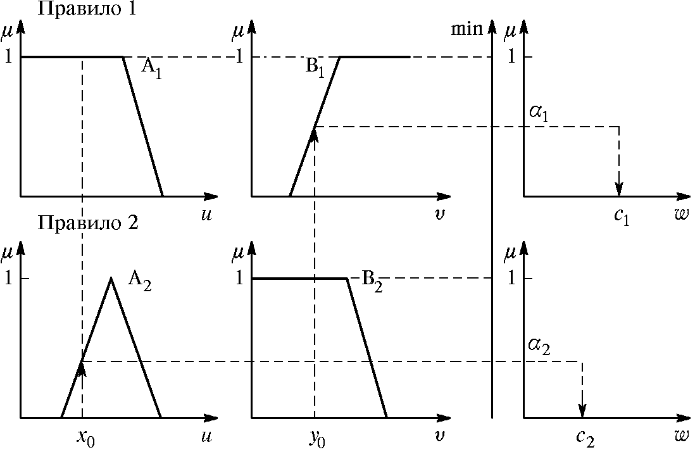
\includegraphics[width=120mm]{fig/algo_simple}
  }
  \caption{Иллюстрация упрощенного алгоритма \\ нечеткого вывода}
  \label{fig:algo_simple}
\end{figure}